\documentclass[a4paper]{article}

\usepackage{fullpage} % Package to use full page
\usepackage{parskip} % Package to tweak paragraph skipping
\usepackage{amsmath}
\usepackage{hyperref}
\usepackage{amsmath,amsfonts,amsthm} % Math packages
\usepackage{graphicx}
\usepackage{listings}
\usepackage{color}
\usepackage{float}
\definecolor{codegreen}{rgb}{0,0.6,0}
\definecolor{codegray}{rgb}{0.5,0.5,0.5}
\definecolor{codepurple}{rgb}{0.58,0,0.82}
\definecolor{backcolour}{rgb}{0.95,0.95,0.92}
\definecolor{brown}{rgb}{0.59, 0.29, 0.0}
\definecolor{beaublue}{rgb}{0.74, 0.83, 0.9}
\definecolor{orange}{rgb}{1.0, 0.5, 0.0}
\definecolor{darkslategray}{rgb}{0.18, 0.31, 0.31}
\def\Xint#1{\mathchoice
	{\XXint\displaystyle\textstyle{#1}}%
	{\XXint\textstyle\scriptstyle{#1}}%
	{\XXint\scriptstyle\scriptscriptstyle{#1}}%
	{\XXint\scriptscriptstyle\scriptscriptstyle{#1}}%
	\!\int}
\def\XXint#1#2#3{{\setbox0=\hbox{$#1{#2#3}{\int}$}
		\vcenter{\hbox{$#2#3$}}\kern-.5\wd0}}
\def\dashint{\Xint-}

% Swap the definition of \abs* and \norm*, so that \abs
% and \norm resizes the size of the brackets, and the 
% starred version does not.
\makeatletter
\let\oldabs\abs
\def\abs{\@ifstar{\oldabs}{\oldabs*}}
%
\let\oldnorm\norm
\def\norm{\@ifstar{\oldnorm}{\oldnorm*}}
\makeatother
\lstdefinestyle{mystyle}{
	backgroundcolor=\color{white},   
	commentstyle=\color{codegreen},
	keywordstyle=\color{blue},
	identifierstyle=\color{brown},
	numberstyle=\tiny\color{codegray},
	stringstyle=\color{orange},
	basicstyle=\footnotesize,
	breakatwhitespace=false,         
	breaklines=true,                 
	captionpos=b,                    
	keepspaces=true,                 
	numbers=left,                    
	numbersep=5pt,                  
	showspaces=false,                
	showstringspaces=false,
	showtabs=false,                  
	tabsize=2
}
\lstset{style=mystyle}

\title{AMATH 569: Problem Set 1}
\author{Jithin D. George, No. 1622555}
%\date{23/11/16}
% matrix environment
\newenvironment{mat}{\left[ \begin{array}{ccccccccccccc}}{\end{array}\right]}
\newcommand\bcm{\begin{mat}}
	\newcommand\ecm{\end{mat}}

\begin{document}

\maketitle
\begin{enumerate}

	
	\item We have 
	\[ u_t +a u_x + b u_y = f\]
	We know
	\[ \frac{du}{dt} = \frac{\partial u}{\partial t} + u_x \frac{dx}{dt} + u_y \frac{dy}{dt}  \]
	Comparing the above two equations, we get, along the curves satisfying
	\[\frac{dx}{dt} =a\]
	\[\frac{dy}{dt} =b\]
	we have
\[\frac{du}{dt} =f\]
\item
 \[ u_t + tu u_x =0 \]
 
 Since this is homogeneous, along the characteristics, u = $u_0(x_0)$
 \[\frac{dx}{dt} = t u\]
 Integrating,
 \[x = \frac{1}{2}t^2 u_0 + x_0 \tag{1}\]
  \[x_0 =x - \frac{1}{2}t^2 u_0 \] 
 Since u is constant along it,
 \[u(x,t) = u(x_0,0)=cos(x - \frac{1}{2}t^2 u)\]
 
 To find breaking time, we differentiate (1) w.t.r t ,
  \[0 = t u + \frac{1}{2}t^2 u_{x_0}{x_0}_{t} +{x_0}_{t} \]
  \[{x_0}_{t} = \frac{-ut}{\frac{1}{2}t^2 u_{x_0} +1}  \]
  
  At breaking time, this is infinite.
  So, 
  \[ t* = \sqrt{\frac{-2}{ u_{x_0}}}= \sqrt{\frac{-2}{ cos(x_0)}}\]
  The minimal realistic (positive) breaking time is t* = $\sqrt{2}$
 
 We can see the characteristics crossing somewhere close to 1. 
\begin{figure}[h!] 
	\centering
	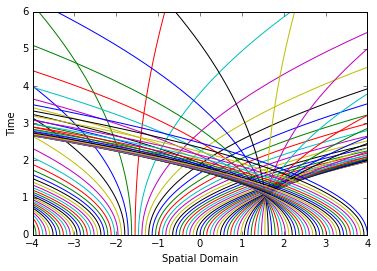
\includegraphics[width=8cm]{q_2.png}

\end{figure}

 
 \item
 \[ u_t + x u_x =0 \]
 

 \[\frac{dx}{dt} = x\]
 Integrating,
 \[x = x_0 e^t \tag{2}\]
 \[x_0 =x e^{-t} \]

  Since this is non-homogeneous, along the characteristics, 
  \[\frac{du}{dt} =1\]
  \[u(x,t)=t + e^{x_0} \]
  \[u(x,t)=t + e^{x e^{-t}} \]

 To find breaking time, we differentiate (2) w.t.r t ,
 \[0 = x_0 e^t + {x_0}_t e^t\]
 \[{x_0}_{t} = - x_0 \]
 
 This does not blow up. 
  Differentiating (2) w.t.r x , we get
  \[{x_0}_{x} = e^{-t} \]
  
  Since this does not go to infinity either, we can say that the characteristics do not cross. This is further confirmed by the plots below.
  
 \begin{figure}[H] 
 	\centering
 	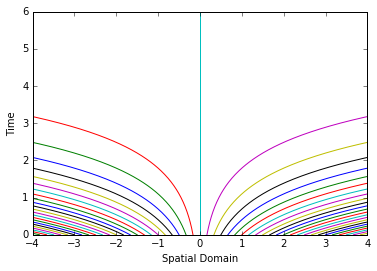
\includegraphics[width=8cm]{q_4.png}
 	
 \end{figure}

\item
\[ u_t + u u_x =0 \]

Since this is homogeneous, along the characteristics, u = $u_0(x_0)$
\[\frac{dx}{dt} =  u\]
Integrating,
\[x = t u + x_0 \tag{3} \]
\[x_0 =x - t u \]
Since u is constant along it,
\[u(x,t) = u(x_0,0)=u(x - t u,0)\]

Differentiating (3) w.t.r x,
\[ {x_0}_x = \frac{1}{u_{x_0} t + 1}\]

For this to be infinite,
\[t = \frac{1}{u_{x_0} }\]



	\begin{enumerate}
		
	\item \[u(x,0)= -x\]
	\[u(x,t) = u(x_0,0)=u(x - t u,0) =tu-x \]
	\[u(x,t) = =\frac{-x}{1-t} \]
	\[u(x,0)= -x\]
\[u_{x_0} = -1\]

\[t* = 1\]	 
Thus, we have the same realistic breaking time for all characteristics as shown below.
 \begin{figure}[H] 
 	\centering
 	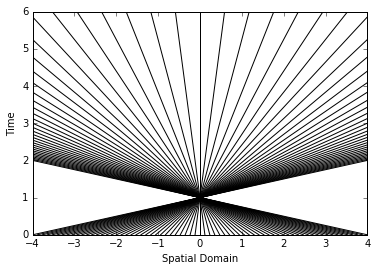
\includegraphics[width=8cm]{5_1.png}
 	
 \end{figure}
\item \[u(x,0)= 1-x^2\]
	\[u(x,t) = u(x_0,0)=u(x - t u,0) =1- (x-tu)^2 = 1-x^2 -t^2u^2+2tux \]
	\[t^2u^2+ (1-2t)u+ x^2-1=0 \]
	\[u(x,t)= \frac{2t-1 \pm \sqrt{(1-2t)^2-4(x^2-1)t^2}}{2t^2} =\frac{2t-1 \pm \sqrt{(1-4t-4x^2t^2+8t^2}}{2t^2} \]
\[u_{x_0} = -2x\]

\[t* = \frac{1}{2x}\]	 
The minimal realistic breaking time goes to 0 as x goes to infinity.
\[ t* =0 \]

This means the solution is invalid for all time. This agrees for our multivalued result for u. (One of them has to be non-physical)
 \begin{figure}[H] 
 	\centering
 	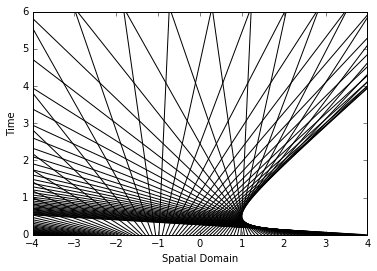
\includegraphics[width=8cm]{5_2.png}
 	
 \end{figure}
\item \[u(x,0)= sin(x)\]
	\[u(x,t) = u(x_0,0)=u(x - t u,0) =sin(x-tu) \]
\[u(x,0)= sin(x)\]
\[u_{x_0} = cos(x)\]

\[t* = \frac{-1}{cos(x)}\]	 
The minimal realistic breaking time is 1 when cos(x) is -1.
\[ t* =1 \]

 \begin{figure}[H] 
 	\centering
 	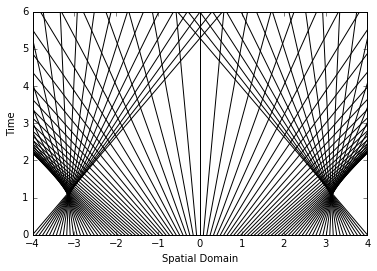
\includegraphics[width=8cm]{5_3.png}
 	
 \end{figure}

	\end{enumerate} 

	\end{enumerate} 
\end{document}